\capitulo{5}{Aspectos relevantes del desarrollo del proyecto}

\section{Inicio del proyecto}
Este proyecto se presentó como un proyecto de investigación sobre la extracción de biomarcadores de la voz para la detección de enfermedades neurodegenerativas o depresión. Al principio, se carecía de un objetivo concreto, debido a la incertidumbre inicial de qué camino se debía seguir y cómo iba a estar de avanzado este área de investigación.

Tras recopilar información, tanto de artículos científicos, como de otras fuentes, se llegó a la conclusión de que el objetivo del proyecto era mejor que estuviera relacionado con la enfermedad del Parkinson. Valoramos diferentes enfermedades como alzheimer, depresión y esclerosis lateral amiotrófica (ELA). Elegimos la enfermedad del Parkinson debido a que la investigación de la detección de esta enfermedad a través de la voz estaba más avanzada y hay muchos artículos recientes y noticias de la realización actual de proyectos en este campo. 

\section{Investigación del proceso a seguir}
Una vez establecida la enfermedad decidimos el proceso a seguir para conseguir un modelo correcto de clasificación de la enfermedad. El proceso a grandes rasgos estaba claro: extraer características de audios y utilizarlas para crear un clasificador. Pero antes, había que decidir varios puntos importantes en el proceso a seguir: ¿De qué audios se deben extraer las características? ¿De dónde íbamos a obtener esos audios? ¿Qué tipo de pre-procesamiento requieren los audios? ¿Qué características se sacan de cada uno de ellos?...

Antes de todo, cabe destacar que como uno de los objetivos era hacer un estudio de investigación sobre diferentes algoritmos para la clasificación de los audios, necesitamos obtener un conjunto de audios de un proyecto concreto para poder comparar nuestros resultados de manera objetiva con ese proyecto concreto. Por ello, el proceso que íbamos a seguir podía estar influenciado de manera directa por el conjunto de datos que se nos prestara.

A la hora de intentar responder a las anteriores preguntas, nos documentamos a través de los artículos más importantes en este campo, con el objetivo de obtener las ideas más relevantes de cada uno de ellos, para decidir el enfoque de nuestro proceso. Los grupos de investigación más importantes se correspondían con dos grupos diferentes de investigadores, los cuales tienen artículos relevantes sobre este tema. La explicación en detalle se dará en el apartado \textit{Trabajos Relacionados} \ref{cap:TrabRel}, sin embargo aquí haremos eco de las ideas más importantes.
Un grupo es el compuesto por Max A. Little y Tsanas Thanasis con artículos como \cite{MxLtSuitability}. Se puede obtener una serie de ideas principales de este grupo:
\begin{itemize}
\item Utilizan únicamente audios de \textbf{vocales sostenidas} para la obtención de características.
\item Sostienen que un conjunto pequeño de características (<20) es suficiente para una correcta clasificación de los audios. Incluso \cite{MxLtNovel} está relacionado íntimamente con esta idea, ya que a partir de un conjunto grande de características utiliza diferentes técnicas de selección de características y demuestra que con un conjunto menor que 20 se obtienen buenos resultados.
\end{itemize}

Otro grupo, también destacado, es el de J. R. Orozco-Arroyave J. D. Arias-Londoño y J. F. Vargas-Bonilla, con artículos como \cite{Orz2016}. La idea más importante que podemos obtener es la siguiente:
\begin{itemize}
\item La pronunciación de \textbf{consonantes en discurso corrido} (frases, textos, palabras...) \textbf{aporta mucha información} de la pronunciación debido a la intervención de diferentes músculos necesarios para ésta. Por ello, se deben analizar otros tipos de audios para obtener más información que si analizamos únicamente pronunciación de vocales sostenidas.
\item Cada tipo de audio debe ser utilizado para hacer un clasificador diferente. No se pueden utilizar diferentes tipos de audio dentro del mismo clasificador, ya que obtenemos resultados confusos, derivados de las diferentes pronunciaciones de diferentes palabras, frases, etc.
\end{itemize}


\begin{tcolorbox}
Condensando ambas, llegamos a la conclusión de que debíamos analizar diversa variedad de audios (ya que aportan más información) sin obsesionarnos por obtener un número inmenso de características de cada uno. Por ello obtendremos variedad de clasificadores que se corresponderán con la variedad de tipos de audio que tengamos y haremos un estudio sobre ellos. Los temas de qué audios utilizar, como pre-procesarles o que características obtener de cada uno se abordará en los siguientes apartados.
\end{tcolorbox}

También se realizó una investigación de todas las posibles características a extraer de los audios y todas las posibles herramientas con las que extraer esas características. Como resultado de esta investigación se crearon una serie de taxonomías, incluidas en el \textbf{anexo de investigación}, en donde se resumen:
\begin{itemize}
\item Artículos relacionados con el tema con información del mismo.
\item Bases de datos encontradas en el estado del arte con información de las mismas (privacidad, características...).
\item Características que se sacan de cada tipo de audio, con información del artículo donde están descritas.
\item Características que se sacan en cada artículo con información sobre ellas.
\item Relación Bibliotecas-Características y viceversa.
\end{itemize}


\section{Conjunto de audios}
El conjunto de datos de audios usado es el descrito en \cite{OrzCorpus}. Como se explica en el artículo, es un conjunto de audios en castellano de 100 personas: 50 de ellas pacientes con Parkinson (PD \footnote{Parkinson Disease}) y 50 de ellas personas sanas, pacientes de control (HC \footnote{Healthy Control}). Es un conjunto de datos realizado de la manera más balanceada posible, a parte de contener 50PD-50HC, también está balanceado en cuanto a sexo y edad tanto dentro de los 50 PD como dentro de los 50 HC. Todos los pacientes han sido diagnosticados por expertos. Se recoge en un arcivo \textit{excel} las características de los audios: edad, sexo, tiempo desde la diagnosis y 3 diferentes medidas: PD/HC (sano o Parkinson), UPDRS-III \cite{updrs} y  Hoehn \& Yahr scale \cite{hoehn1967}. Como se ha visto en \ref{sec:Updrs} , tanto UPDRS como Hoehn \& Yahr son dos escalas utilizadas para medir la severidad del Parkinson.

El conjunto de audios contiene un total de 4200 audios tipo wav, divididos en los siguientes tipos:
\begin{description}
	\item[Monólogos] 50 monólogos de PD y 50 de HC. El contenido es discurso libre sobre la respuesta a la pregunta \textit{¿Qué haces cuando te levantas por la mañana?}. La duración de este tipo de audios comprende desde 00:30 a 02:30.
	\item[Texto leído] 50 audios de PD y 50 de HC. El contenido es el siguiente texto balanceado: \textit{Ayer fui al médico. ¿Qué le pasa? Me preguntó. Yo le dije: Ay doctor! Donde pongo el dedo me duele. ¿Tiene la uña rota? Sí. Pues ya sabemos qué es. Deje su cheque a la salida.}
	\item[Vocales] 750 audios de PD y 750 de HC. Pronunciación sostenida de cada una de las 5 vocales 3 veces por persona. 150 audios de HC y 150 de PD por cada vocal.
	\item[Palabras] 1250 audios de PD y 1250 de HC. Pronunciación de palabras para el análisis silábico. Cada persona tanto PD como HC pronunciará 25 palabras diferentes: \textit{brasa, coco, petaca, etc}.
\end{description}

\section{Metodología del estudio - Resumen general}
En esta sección se hará una mera introducción inicial al estudio realizado, explicado más adelante en las siguientes secciones y mucho más detallado en los \english{notebooks} del proyecto. En estos \textit{notebooks} se detallan tanto detalles de implementación, como detalles de uso, como detalles de análisis de resultados y del proceso de la investigación. Los notebooks se encuentran tanto en el directorio \filename{/src} como en el directorio \filename{/src/vggish}. A lo largo de esta sección, se irán detallando en qué \textit{notebooks} aparece cada experimento o cada extracción de características.

Un aspecto importante del proyecto es el siguiente. En un primer momento se planeó la extracción de características, creación de los clasificadores y finalmente utilización de ellos. Para ello comenzamos, en la \textbf{primera fase} de experimentos, extrayendo las características (que comentaremos posteriormente) con la biblioteca \textbf{Disvoice}. Ésta es una herramienta pública desarrollada por el mismo grupo de investigación del artículo \cite{Orz2016}. Creamos los diferentes clasificadores para esas características y obtuvimos resultados inferiores a los recogidos en el estado del arte, i.e. \cite{Orz2016}. Obtuvimos resultados inferiores a pesar de usar los mismos clasificadores con los mismos parámetros y de mantener conversaciones con los autores para resolver posibles ambigüedades sobre las herramientas o el proceso utilizado. Destacamos que en las diferentes fases del estudio, lo que hemos ido variando han sido los conjuntos de datos extraídos de cada audio, realizando los mismos experimentos con clasificadores (o modificando los experimentos muy poco).

Como no obtuvimos los resultados esperados, decidimos hacer una mejora a los experimentos, una \textbf{segunda fase} del estudio. Esta mejora consistía en dos partes. La primera de ellas fue añadir para cada instancia los atributos \textbf{edad y sexo} del paciente a las características extraídas por \textit{Disvoice}. Estos datos les tenemos disponibles en el archivo \textit{excel} descrito en \cite{OrzCorpus}, que se nos envió junto con los audios cortesía de J.R Orozco-Arroyave de la Universidad de Antioquía, Colombia. La segunda mejora fue separar las instancias del conjunto de datos entre hombres y mujeres. Se planteó de esta manera, debido a que \cite{Orz2016} hace validación cruzada estratificada según dos elementos: edad y clase (PD: \english{Parkinson Disease} o HC: \english{Healthy control}). Con la biblioteca utilizada para los experimentos, \english{scikitlearn}, solamente se puede estratificar según 1 atributo. Separando los conjuntos de datos por sexos y estratificando cada sexo por clase, estamos simulando esa validación cruzada estratificada por 2 atributos que utiliza ese artículo. Se mejoraron los resultados obtenidos con los conjuntos de datos de la primera fase, pero aun así estaban lejos de los resultados en el estado del arte.

Con intención de mejorar los resultados y dar una perspectiva diferente a los experimentos, realizamos una \textbf{tercera fase} de los mismos. En esta tercera fase utilizamos la biblioteca de \english{Deep Learning} llamada \textbf{VGGish} \cite{vggish} (ver sección \label{subsec:vggish}). Consiste en la extracción de características mediante la una red neuronal pre-entrenada con audios de \english{Youtube},  que utiliza capas convolucionales. Al estar pre-entrenada, ya tenemos los pesos para la extracción de características y, por tanto, lo único que debemos realizar es utilizar las funciones de extracción de esa biblioteca. En esta fase, sacamos para cada audio otros dos conjuntos de características, \textit{embeddings} de \textit{VGGish} (media y desviación de \textit{embeddings}, se explicará en \ref{sec:fase3}) y espectros de frecuencia, con los cuales realizamos los experimentos con los clasificadores. Los resultados obtenidos seguían estando en la magnitud de los obtenidos por nosotros, pero sin llegar a los mejores del estado del arte.

Cabe destacar que en todos ellos se ha realizado una validación cruzada con 10 \textit{folds}, ya que es la que se utiliza en \cite{Orz2016} o \cite{MxLtAccurate}. También destacamos que la medida que hemos utilizado para los clasificadores es el área bajo la curva ROC, \filename{roc\_auc\_score} en \english{Scikit-Learn}. Esto es debido al siguiente motivo. Lo más óptimo hubiera sido extraer tanto el área bajo la curva, como el \english{accuracy}, como otras medidas. Sin embargo, en las clases creadas por nosotros (experimenters y funciones de realización de experimentos), no se pueden extraer multimétricas de los experimentos, si queremos extraer dos métricas diferentes, se debe realizar otra vez el experimento indicando que se devuelve la otra métrica. Debido a la cantidad de experimentos realizada, hemos decidido que la mejor medida era el área bajo la curva ROC. Es debido a que si obtenemos altas magnitudes de esta medida, aunque después medidas como la \english{accuracy} no sean tan altas, lo único que debemos hacer el elegir correctamente cual es el umbral de decisión del clasificador. Es decir, elegir a partir de qué probabilidad de clase predicha por el clasificador, nuestra instancia es de una clase o de la otra. El último aspecto a destacar es que todos los experimentos han sido realizados en \english{notebooks} de \textit{Jupyter}. Se ha considerado que es el entorno interactivo más idóneo para la realización y presentación de experimentos. En todos estos \english{notebooks} se realiza una explicación detallada de los experimentos y, también, una visualización de resultados con multitud de gráficas y tablas para su mejor análisis y comprensión. Algunos de los resultados más importantes se encuentran en la sección \ref{sec:resultados}.

Tras finalizar todos estos experimentos con todos los diferentes conjuntos de datos extraídos de los audios, realizamos una aplicación de escritorio con \textit{tkinter}, en la que se muestre cómo podría aplicarse el resultado de investigación a un producto final. En ella se podrá analizar un audio y, tras procesarlo, que nos diga la probabilidad de que la persona de ese audio tenga Parkinson o no, y se muestren las gráficas de amplitud de onda y de espectrograma de frecuencias.



\section{Primera Fase: atributos Disvoice}
Nuestro estudio comprenderá la comparación de diferentes clasificadores construidos cada uno con diferentes conjuntos características para cada tipo de audio. Utilizaremos 3 diferentes tipos de audio: \textbf{vocales sostenidas, 5 palabras diferentes y texto leído}. Qué características sacamos para cada tipo de audio se presentará en la subsección \textit{Modelado del discurso} \ref{subs:modeldisc}. El proceso para la realización de los clasificadores es el siguiente (ver Figura \ref{fig:proceso}):
\begin{enumerate}
\item Pre-procesamiento de los audios: preparación de audios para la extracción de diferentes medidas.
\item Modelado del discurso: extracción de diferentes tipos de características para cada tipo de audios.
\item Clasificación: construir diferentes clasificadores para cada conjunto de características para hacer un estudio comparativo.
\end{enumerate}

\begin{figure}[!h]
		\centering
		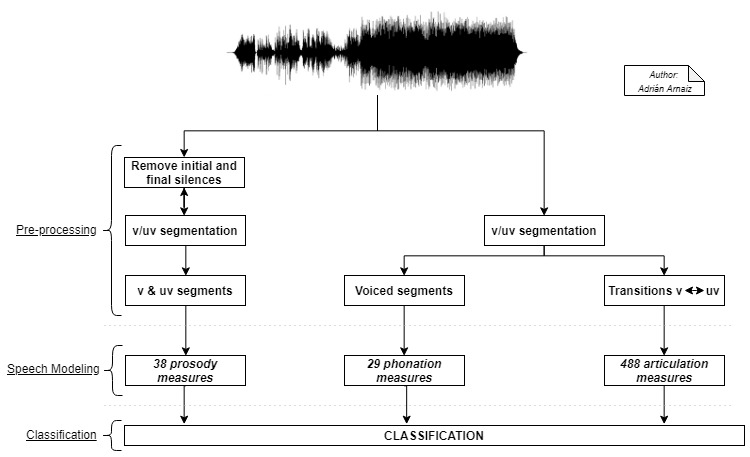
\includegraphics[width=0.9\textwidth]{proceso}
		\caption[Esquema del proceso para abordar los experimentos.]{Esquema del proceso para abordar los experimentos, basada en \cite{Orz2016}}\label{fig:proceso}
\end{figure}

\subsection{Pre-procesado de audios}
En esta etapa se realizan 2 tareas principales: la eliminación de silencios iniciales y finales de los audios y la segmentación en fragmentos con voz y sin voz de los mismos (los llamaremos segmentos \english{voiced} y \english{unvoiced}).
La eliminación de sonidos inicial y final de los audios se realiza ya que a la hora de extraer las medidas de prosodia se puede tener algunos inconvenientes si los silencios iniciales son muy largos. Si fueran excesivamente largos tendríamos resultados erróneos en las características, como, por ejemplo, las relacionadas con la duración promedio de silencios, la variabilidad de la duración de los silencios y otras medidas que se calculan sobre las pausas.
Para la extracción de medidas de fonación y articulación este proceso lo realizan internamente los \english{scripts} de la biblioteca \textit{Disvoice} \cite{neurospeech} utilizando \textit{Praat}. Sin embargo, a la hora de obtener las medidas prosódicas es necesario realizar la eliminación de manera previa.

La \textbf{segmentación en fragmentos \english{voiced} y \english{unvoiced}} se realiza para analizar el discurso, es decir, se sacarán medidas que necesitan de esta fragmentación (i.e. \english{Jitter} de los fragmentos \english{voiced} o MFCC de las transiciones entre \english{voiced} y \english{unvoiced}). Esta tarea la hacen internamente los \english{scripts} de la biblioteca \textit{Disvoice} utilizando \textit{Praat}.

\subsection{Modelado del discurso} \label{subs:modeldisc}
Se extraerán, con la herramienta \textit{Disvoice}, 3 diferentes conjuntos de características para cada tipo de audio: de fonación, de articulación y prosódicas. Como hemos visto en nuestro conjunto de datos, tenemos texto leído, palabras, vocales y monólogos. En este proyecto utilizaremos el texto leído, las 5 palabras con mejor resultado en \cite{Orz2016} (\textit{atleta, campana, braso, gato, petaca}) y las 5 vocales. El monólogo no será utilizado debido a que al ser discurso libre y no predefinido, las características extraídas dependen también de cómo sea el discurso (i.e. las palabras que se digan, las pausas...). También se realizará la limpieza de las características, en nuestro caso, tratar los datos de tipo \textit{NaN} resultantes en la extracción. Como se ve en los \english{notebooks} de extracción de características y se comentará posteriormente, se decidió por eliminar las instancias que contienen \textit{NaN}, ya que no eran muchas.

La extracción de estas características se encuentra realizada y explicada en el \textit{notebook} de la ruta \filename{TFG-Neurodegenerative-Disease-Detection/src/  Extracción de características.ipynb}.


\subsubsection{Medidas de fonación}
De las medidas de fonación obtendremos 11 conjuntos diferentes: 1 para el texto leído, 5 para las palabras (1 por palabra elegida) y 5 por vocal (1 por vocal). En total, de cada audio se sacan un conjunto de \textbf{29 medidas} basadas en la perturbación de la fonación. Las medidas de fonación, son extraídas de los segmentos \english{voiced}, utilizando para ello la biblioteca Disvoice (\filename{phonation.py}). Estas características son descritas en la tabla \ref{tabla:ccasfonacion}.

\tablaSmall{Características de fonación.  En detalle en \cite{neurospeech}.}{l c c}{ccasfonacion}
{ \multicolumn{1}{l}{Caract.} & Número & Breve descripción\\}{ 
1ª derivada F0 & 1$\times$4=4 & 1ª deriv. frec fundamental\\
2ª derivada F0 & 1$\times$4=4 & 2ª deriv. frec fundamental\\
Jitter & 1$\times$4=4 & Perturbación de F0\\
Shimmer & 1$\times$4=4 & Perturbación de Amplitud\\
APQ & 1$\times$4=4 & Cociente de perturb. de amplitud\\
PPQ & 1$\times$4=4 & Cociente de perturb. de periodo\\
Energía Log & 1$\times$4=4 & Explicado en \cite{etsi} \\
Grado unvoiced & 1 & Grado \english{unvoiced}\\
} 

\begin{tcolorbox}
Obtenemos un vector de 29 características, las descritas en la tabla \ref{tabla:ccasfonacion}: las 7 medidas por sus 4 funcionales (media \textit{m}, desviación \textit{std}, curtosis \textit{k} y oblicuidad \textit{sk}) + grado de \textit{unvoiced} \footnote{El grado de unvoiced es el ratio entre la duración de los segmentos sin voz entre la duración total del audio \cite{neurospeech}.}.
\end{tcolorbox}


\subsubsection{Medidas de articulación}\label{subsubsec:articulacion}
De las medidas de articulación obtendremos 6 conjuntos diferentes: 1 para el texto leído y 5 para las palabras (1 por palabra elegida). En total de cada audio se sacan un conjunto de \textbf{488 medidas} de articulación. Las medidas de articulación son extraídas de las  transiciones entre los segmentos \english{voiced} y \english{unvoiced} utilizando para ello la biblioteca Disvoice (\filename{articulación.py}). Estas características son descritas en la tabla \ref{tabla:ccasarticulacion}

\tablaSmall{Características de articulación. En detalle en \cite{neurospeech}.}{l c c c}{ccasarticulacion}
{ \multicolumn{1}{l}{Caract.} & Número & Breve descripción\\}{ 
BBE onset & 22$\times$4=88 & 22 coef. BBE de trans. \textit{v} -> \textit{uv}\\
MFCC onset & 12$\times$4=48 & 12 coef. MFCC de trans. \textit{v} -> \textit{uv}\\
1ªD MFCC onset & 12$\times$4=48 & 1ª deriv. 12 coef. MFCC de trans. \textit{v} -> \textit{uv}\\
2ªD MFCC onset & 12$\times$4=48 & 2ª deriv. 12 coef. MFCC de trans. \textit{v} -> \textit{uv}\\
BBE offset & 22$\times$4=88 & 22 coef. BBE de trans. \textit{uv} -> \textit{v}\\
MFCC offset & 12$\times$4=48 & 12 coef. MFCC de trans. \textit{uv} -> \textit{v}\\
1ªD MFCC offset & 12$\times$4=48 & 1ª deriv. coef. 12 MFCC de trans. \textit{uv} -> \textit{v}\\
2ªD MFCC offset & 12$\times$4=48 & 2ª deriv. coef. 12 MFCC de trans. \textit{uv} -> \textit{v}\\
1ª formante F0 & 1$\times$4=4 & 1ª formante de frecuencia  \\
1ªD 1ª formante F & 1$\times$4=4 & 1ª deriv. 1ª formante de frecuencia \\
2ªD 1ª formante F & 1$\times$4=4 & 2ª deriv. 1ª formante de frecuencia \\
2ª formante F & 1$\times$4=4 & 2ª formante de la frecuencia \\
1ªD 2ª formante F & 1$\times$4=4 & 1ª deriv. 2ª formante de frecuencia \\
2ªD 2ª formante F & 1$\times$4=4 & 2ª deriv. 2ª formante de frecuencia \\

} 

\begin{tcolorbox}
Obtenemos un vector de 488 características, las descritas en la tabla \ref{tabla:ccasarticulacion}: las 122 medidas por sus 4 funcionales(media \textit{m}, desviación \textit{std}, curtosis \textit{k} y oblicuidad \textit{sk}).
\end{tcolorbox}


\subsubsection{Medidas de prosodia}
De las medidas de prosodia obtendremos 1 conjuntos para el texto leído. En total de cada audio se sacan un conjunto de \textbf{38 medidas} basadas en la duración, la frecuencia fundamental, la energía y ratios de la composición del audio en lo relativo a segmentos \english{voiced} y \english{unvoiced}. Las medidas de prosodia son extraídas del audio completo, tanto segmentos \english{voiced} como \english{unvoiced}, utilizando para ello la librería Disvoice (\filename{prosodia.py}). Estas características son descritas en la tabla \ref{tabla:ccasprosodia}.

\tablaSmall{Características de prosodia. En detalle en \cite{neurospeech}.}{l c c c}{ccasprosodia}
{ \multicolumn{1}{l}{Caract.} & Número & Breve descripción\\}{ 
Frec. fundamental & 7 & relativas a la frec. fundamental\\
Energía & 9  & 9 medidas relativas a la energía\\
Ratios \textit{v}-\textit{uv} & 22  & 22 medidas relativas a \textit{v}-\textit{uv}\\
}

\begin{tcolorbox}
Obtenemos un vector de 38 características, las descritas en la tabla \ref{tabla:ccasprosodia}. Esta vez sin sacar los funcionales para cada medida.
\end{tcolorbox}

\subsubsection{Conjuntos de datos totales} \label{subsubsec:datos}
En total tenemos \textbf{18} conjuntos diferentes de características: medidas de fonación articulación y prosodia para la frase, medidas de fonación y articulación para cada una de las palabras y medidas de fonación para las vocales sostenidas. Se construyen clasificadores independientes para cada subconjunto diferentes, como hemos comentado anteriormente, no se pueden mezclar características extraídas de diferentes frases, palabras o vocales, ya que hay características intrínsecas a la pronunciación de esos elementos. Cada conjunto de características se ha extraído en \english{scripts} en \english{notebooks} de \textit{Python}, utilizando métodos de clases que envuelven el funcionamiento de la biblioteca \textit{Disvoice}. Los conjuntos de datos extraídos de vocales y palabras tienen 100 instancias con N atributos, siendo N el número de atributos descrito en las 3 anteriores subsecciones. Los conjuntos extraídos de las vocales tienen 300 instancias, ya que para cada vocal tenemos 3 audios distintos. Para cada conjunto de características se ha creado una función del mismo estilo que los cargadores de datos de \english{Scikit-Learn}: funciones dentro de módulos que devuelven objetos de tipo \english{Bunch}. Además, cada conjunto de datos tiene un nombre del estilo (fon|art|prs)\_(rt|w\_palabra|v\_vocal)\_ccas y se guardan en formato \textit{numpy} en el directorio \filename{src/CaracteristicasExtraidas}. 

Explicación de la nomenclatura:
\begin{description}
\item[fon] Fonación.
\item[art] Articulación.
\item[prs] Prosodia.
\item[rt] Frase, \english{read-text}.
\item[w\_palabra] Palabra, i.e. \textit{fon\_w\_gato\_ccas} o \textit{art\_w\_braso\_ccas}.
\item[v\_vocal] Vocal, i.e. \textit{fon\_v\_A\_ccas} o \textit{art\_v\_E\_ccas}.
\end{description}

\subsection{Experimentos con clasificadores}\label{subs:expprimfase}
Los experimentos de esta fase se encuentran realizados y explicados en el \english{notebook} alojado en \filename{TFG-Neurodegenerative-Disease-Detection/src/1os Experimentos clasificadores.ipynb}. Para todos los conjuntos de datos se han realizado varios tipos de experimentos, comprendiendo desde los clasificadores estándar de \english{Scikit-Learn}, hasta métodos más complejos de \english{bagging} o \english{boosting} con pre-procesado de datos (normalización), selectores de características (\english{select k best, variance treshold...}), búsquedas exhaustivas de parámetros... 

Los experimentos realizados han sido los siguientes:
\begin{itemize}
\item  Experimento con clase \filename{experimenter}. Esta es una clase implementada por nosotros, que, explicada a grandes rasgos, dados unos conjuntos de datos y clasificadores pasados como un diccionario, realiza todos los pares de experimentos devolviendo todos los resultados. Los conjuntos de datos serán los 18 descritos anteriormente y los clasificadores serán 8 clasificadores diferentes de \english{Scikit-Learn} con sus valores por defecto y sin ningún elemento de selección de atributos o búsqueda de parámetros. Obtenemos una tabla de resultados de 144 resultados de los 144 experimentos diferentes. El AUC más alto obtenido es de \textbf{0.836}, obtenido con el método \textit{AdaBoost} para el conjunto de datos de fonación de la frase (\english{read\_text}).
\item Experimento llamado \textit{Orozco} ya que es el experimento realizado en \cite{Orz2016}. Consiste en utilizar el algoritmo de clasificación SVM con kernel gaussiano, con una búsqueda exhaustiva de los parámetros C y lambda. Por ello hemos implementado un \english{grid search} con \english{Scikit-Learn}. El mejor resultado es de \textbf{0.744} AUC para las características de fonación de la vocal U. Muy lejos del 0.99 AUC y 0.99 \english{accuracy} que se obtiene en \cite{Orz2016} con el mismo experimento.
\item Reducción de dimensionalidad PCA, con clasificador SVM y búsqueda de parámetros. Se implementa un \english{pipeline} que contiene todos esos pasos del experimento. El mejor resultado es de \textbf{0.76} AUC para las características de fonación de la vocal U.
\item AdaBoost con búsqueda de parámetros del número de estimadores. El mejor resultado es de \textbf{0.832} AUC para las características de fonación de la frase.
\item Selección de atributos con \english{variance threshold} para diferentes clasificadores. El mejor resultado es de \textbf{0.884} AUC, con AdaBoost, para las características de fonación de la frase.
\item Selección de atributos con el método K best, con el clasificador AdaBoost y con búsqueda de parámetros para el parámetro $k$ del selector. El mejor resultado es de \textbf{0.74} AUC para las características de fonación de la frase.
\item Selección de atributos con el método K best para diferentes clasificadores. El mejor resultado es de \textbf{0.78} AUC para las características de fonación de la palabra gato.
\end{itemize}


\subsection{Resultados}
Vistos los resultados (véase Tabla \ref{tabla:resfase1}), quedan muy lejos de los obtenidos en \cite{Orz2016}. El mejor de los anteriores es el de selección de atributos con \english{variance threshold} para diferentes clasificadores, cuyo resultado es de \textbf{0.884} AUC, con AdaBoost, para las características de fonación de la frase. Se considera que este resultado por el mismo no es malo, pero sí lo es en comparación con el estado del arte. En el \textit{notebook} comentado, se incluyen gráficos de barras y tablas que hacen más vistoso y comprensible el análisis de resultados del experimento.

\tablaSmall{Resumen resultados fase 1.}{l c c}{resfase1}
{ \multicolumn{1}{l}{Exp.} & AUC\\}{ 
Experimenter & 0.836 \\
GS - SVM & 0.744 \\
GS - PCA - SVM & 0.768\\
GS - VT - AdaBoost & 0.832 \\
VT - varios & 0.884  \\
KBest - varios & 0.780 \\
GS - KBest - AdaBoost & 0.744 \\

} 

\subsection{Proyección gráfica de las características}
Realizamos una proyección gráfica de las características de esta fase, para tener una idea de como se distribuyen los datos y tener una visión de si las clases son claramente separables o no. Se realiza en el \english{notebook} alojado en \filename{src/Proyeccion\_ccas\_DisVoice.ipynb}. Como nuestros vectores de características tienen muchos atributos, realizamos la reducción de dimensionalidad con 4 métodos diferentes: análisis de componentes principales (PCA con y sin kernel), TSNE y análisis de discriminante linear (LDA). Llegamos a la conclusión que no hay una separación clara de las clases, únicamente se atisba una ligera separación con el la reducción realizada con el método LDA (ver Figura \ref{fig:proyeccion_lda}).
\imagen{proyeccion_lda}{Proyeccion realizada con LDA.}


\section{Segunda Fase: Disvoice modificado}
Como anteriormente hemos comentado, realizamos modificaciones sobre los datos anteriores con el objetivo de mejorar los resultados de los experimentos. Para ello, lo primero que realizamos fue añadir los atributos edad y sexo del paciente a nuestro vector de características. Por ello, tenemos los mismos 18 subconjuntos de características explicados en \ref{subsubsec:datos}, pero cada instancia con dos atributos más: edad y sexo. Estos atributos fueron añadidos ya que les consideramos importantes a la hora de analizar físicamente la onda de la voz. Evidentemente habrá diferencias en medidas como frecuencias fundamentales o \english{Jitter} entre sexos, o entre personas  mayores y personas jóvenes.

La segunda mejora fue separar las instancias del conjunto de datos entre hombres y mujeres, y realizar clasificadores diferentes para cada grupo. Se planteó de esta manera, debido a que \cite{Orz2016} hace validación cruzada estratificada según dos elementos: Edad y clase (PD: \english{Parkinson Disease} o HC: \english{Healthy control}). Con la biblioteca utilizada para los experimentos, \english{Scikit-Learn}, solamente se puede estratificar según 1 atributo. Separando los conjuntos de datos por sexos y estratificando cada sexo por clase, estamos simulando esa validación cruzada estratificada por 2 atributos que utiliza ese artículo. De esta manera obtenemos los conjuntos de datos de medidas de fonación articulación y prosodia, pero únicamente añadiendo el atributo edad, ya que el atributo sexo no hace falta: debido a la división por sexo todos son el mismo. Un problema que tenemos es que, como nuestros conjuntos de datos son pequeños (100 o 300 instancias), a la hora de dividir son todavía más pequeños: tendremos el doble de conjuntos de datos de la mitad de tamaño (50 0 150 instancias).

Por último, creamos unos conjuntos de datos con únicamente las características MFCC de los audios, estas son un subconjunto de las medidas de articulación (véase \ref{subsubsec:articulacion}), que comprenden únicamente los atributos MFCC y sus dos primeras derivadas. Esto es debido a que son las características con las que mejor resultado se obtiene en el estado del arte, y son exactamente las mismas que las extraídas en \cite{Orz2016}. Así que, para cada audio posible, hemos obtenido este conjunto de características, también dividido por sexo.

Por ello, hemos realizado 3 \english{notebooks} de experimentos en esta segunda fase: Uno para los experimentos con las características \textit{Disvoice} más edad y sexo, otro para las características \textit{Disvoice} de las mujeres más el atributo edad y otro para las características \textit{Disvoice} de los hombres más la edad. Los conjuntos de datos de las características MFCC comentadas como tercera mejora, fueron divididos por sexo y participan en los experimentos de los \english{notebooks} de experimentos con mujeres y de experimentos con hombres.


\subsection{Modelado del discurso}
Se extraen las características de fonación, articulación y prosodia de cada audio comentado anteriormente, y posteriormente se añaden los atributos edad y sexo. La extracción de las características físicas se realiza con la herramienta \textit{Disvoice} al igual que anteriormente. Los atributos edad y sexo se añaden con el extractor de características creado, que añade automáticamente al conjunto de datos los datos extra (en nuestro caso edad y sexo) que contiene un diccionario. Esta clase creada por nosotros, permite tanto añadir esos atributos extra a un conjunto de datos ya extraído, como extraer las características de un audio y añadir esos atributos extra en el propio proceso de extracción directa del audio.

Para la extracción de las características MFCC, como son un subconjunto de las características de articulación, nos fijamos en los índices de las características en la documentación de \textit{Disvoice} y extrajimos esas columnas indicadas.

La extracción de estas características se encuentra realizada y explicada en el \textit{notebook} de la ruta \filename{TFG-Neurodegenerative-Disease-Detection/src/ Extracción de características MODIFICADAS Disvoice.ipynb}.

\subsubsection{Conjuntos de datos totales}
Debido a lo que acaba de ser explicado, tenemos un total de \textbf{78} conjuntos de datos diferentes. 18 de ellos son igual que los de la anterior fase, pero añadiendo los atributos edad y sexo. 30 de ellos son los extraídos con \textit{Disvoice} para las mujeres más la edad (18 anteriores + 12 de características MFCC). Los 30 restantes son los 30 extraídos de los hombres. El número de instancias de cada conjunto de datos varía. Para los divididos por sexo (60 conjuntos diferentes) serán la mitad que los de la primera fase: 50 para las palabras y la frase y 150 para las vocales. En cambio, para los que únicamente hemos añadido edad y sexo (18 diferentes) tendremos las mismas instancias que en la primera fase, 100 o 300. Se construyen clasificadores independientes para cada conjunto de los 78 diferentes, como hemos comentado anteriormente

Las características extraídas se guardan en formato \textit{numpy} en los directorios: \filename{src/CaracteristicasExtraidas/DivisionSexo/hombres,\\ src/CaracteristicasExtraidas/DivisionSexo/mujeres y\\ src/CaracteristicasExtraidas/EdadYSexo.}

\subsection{Experimentos con clasificadores}
Los experimentos de esta fase se encuentran agrupados en 3 \english{notebooks} diferentes. Uno para los experimentos con las características \textit{Disvoice} más edad y sexo, otro para las características \textit{Disvoice} de las mujeres más el atributo edad y otro para las características \textit{Disvoice} de los hombres más la edad. Son los realizados en:
\begin{itemize}
\item \filename{src/2os Experimentos A - Disvoice + Edad y Sexo.ipynb}
\item \filename{src/2os Experimentos B - Disvoice Mujeres.ipynb}
\item \filename{src/2os Experimentos B - Disvoice Hombres.ipynb}
\end{itemize} 
Todos estos documentos contienen explicación detallada de los experimentos y visualización de resultados en multitud de gráficas y tablas para su mejor análisis y comprensión. Para todos los conjuntos de datos se han realizado varios tipos de experimentos al igual que anteriormente. Se han realizado por lo general los mismos experimentos que en la primera fase, con algunos nuevos experimentos en cada \textit{notebook} que íbamos avanzando.

Para los experimentos de las características \textit{Disvoice} más edad y sexo sin dividir por sexos (\filename{TFG-Neurodegenerative-Disease-Detection/src/2os Experimentos A - Disvoice + Edad y Sexo.ipynb}) se han realizado la repetición de los mismos experimentos de la primera fase pero con estos nuevos datos(véase \ref{subs:expprimfase}).

Para los 2 \english{notebooks} de experimentos de las características \textit{Disvoice} divididas por sexos se han realizado la repetición de los mismos experimentos de la primera fase, más u nuevo experimento: Selección de características con K Best, clasificador \english{Gradient Boost Classifier} y búsqueda de parámetros.



\subsection{Resultados}
Por lo general, el AUC de los experimentos ha aumentado debido a los cambios realizados, pero sin ser un incremento muy notable, ni llegar a resultados parecidos a los comentados del estado del arte.
El mejor resultado para los experimentos de las características \textit{Disvoice} más edad y sexo sin dividir por sexos es el de selección de atributos con \english{variance threshold} para diferentes clasificadores, cuyo resultado es de \textbf{0.884} AUC, con AdaBoost, para las características de fonación de la frase. Coincide exactamente con los resultados de la primera fase. Es mera coincidencia, ya que en los demás experimentos, los resultados sí que han variado mejorando muy poco por lo general.

Para los experimentos con las mujeres conseguimos \textbf{el mejor resultado conseguido en todos los experimentos}. Lo hemos conseguido con selección de parámetros con K Best, AdaBoost y búsqueda de parámetros. Conseguimos un \textbf{0.908 AUC} con el conjunto de datos de características de articulación de la palabra \textit{campana}. Cabe destacar que en todos los experimentos con la separación por sexos, se aumenta el rendimiento de los clasificadores: un 0,02 AUC el mejor caso y hasta un 0,05 AUC la media de todos los experimentos. 

Para los experimentos con los hombres no conseguimos tan buen resultado como para las mujeres. El mejor resultado lo hemos conseguido con selección de parámetros con K Best, Gradient Boost Classifier y búsqueda de parámetros. Conseguimos un \textbf{0.867} AUC con el conjunto de datos de características MFCC de la palabra \textit{atleta}, es decir, uno de los nuevos conjuntos de datos que hemos sacado en esta fase.

Los experimentos y resultados al detalle se explicarán de manera más extensa en el anexo de investigación y en los \english{notebooks}. Sin embargo, el resumen de los resultados se puede ver en la tabla \ref{tabla:resfase2}. En las casillas donde no hay resultados, es debido a que los experimentos les hemos realizado de manera adicional en los siguientes pasos (para hombres y mujeres) y no en anteriores \textit{notebooks}.

\tablaSmall{Resumen resultados fase 2.}{l c c c c}{resfase2}
{ \multicolumn{1}{l}{Exp.} & +Ed-Sx & Muj & Hom\\}{ 
Experimenter & 0.836 & 0.894 & 0.813 \\
GS - SVM & 0.721 & 0.725 & 0.769 \\
GS - VT - AdaBoost & 0.860 & 0.905 & 0.838 \\
VT - varios & 0.884 & 0.883 & 0.813 \\
KBest - varios & 0.759 & 0.816 & 0.838 \\
GS - KBest - AdaBoost & - - & \textbf{0.908} & 0.816 \\
GS - KBest - Rand For & 0.748 & 0.820 & 0.816 \\
GS - KBest - GBC & - - & 0.880 & 0.867\\
} 



\section{Tercera Fase: VGGish} \label{sec:fase3}
Como último recurso para mejorar los resultados y, además, dar una nueva visión a la extracción de características, añadimos la innovación al estado del arte de utilizar para la extracción una red neuronal pre-entrenada con capas convolucionales: \concept{VGGish} (véase sección \ref{subsec:vggish}). Esta red ha sido utilizada para extraer características, 128 \english{embeddings} de cada audio. Estos \english{embeddings} no son interpretables. 

A su vez, en esa biblioteca VGGish, también se provee un extractor de las características de estilo MFCC y espectros, ya que es parte del proceso para finalmente sacar los \english{embeddings}. Dado nuestro escepticismo surgido con le herramienta \textit{Disvoice}, debido a los bajos resultados obtenidos comparando con el artículo de los mismos autores \cite{Orz2016}, también hemos generado conjuntos de datos que son MFCC y espectros. Por ello, hemos obtenido otra serie de conjuntos de datos de esta manera.

Cabe destacar que, con el modelo VGGish solo podemos sacar características para los audios de más de 0.975 segundos. Esto se debe al funcionamiento de \textit{VGGish}. Para \textit{VGGish} una instancia es un frame de 0.96s de un audio, no el audio entero. Por ello, saca características para cada ventana de 25ms (por eso el limite de 0.975s) con solapamiento de 10ms. Es decir, todas las palabras y muchas vocales no podrán ser procesadas por este modelo debido a su corta duración (el 99\% de las palabras duran menos de un segundo y algunos audios de las vocales también). Por tanto, realizaremos la extracción de características para la frase y para las vocales que se pueda.


\subsection{Modelado del discurso}
\textit{VGGish} tiene varios pasos. La entrada de la red \textit{VGGish} debe ser una matriz de tamaño 96x64 y la salida un vector unidimensional de tamaño 128. Concretamente, 96 son las ventanas que analiza y 64 las características que saca el pre-procesado de cada ventana. Por ello, el pre-procesado devuelve un array de matrices de 96$\times$64, que servirá de entrada a la red \textit{VGGish}, cada una como ejemplo independiente. Por ello, si hacemos el proceso entero con un audio, al final con \textit{VGGish} obtendremos una matriz de tamaño (duración del audio/0.975)$\times$128. Debido a que la entrada a nuestro modelo deberá ser una instancia, hemos optado por hacer la media y desviación de cada \textit{embedding} obtenido con \textit{VGGish} y así finalmente obtener un vector de tamaño 256. El esquema del proceso es el siguiente:

Audio wav $\rightarrow$ \textbf{|Pre-procesado|} $\rightarrow$ MFCC y espectros para cada 0.96s $\rightarrow$ \textbf{|VGGish|}$\rightarrow$ Embeddings $\rightarrow$ \textbf{|Media y desv|} $\rightarrow$ vector final (size 256)

Como hemos comentado también extraemos las características de estilo MFCC. Por ello, usamos únicamente la etapa de pre-procesado para obtener los datos. Como hemos comentado, nos devuelve array de matrices de 96x64, es decir, devuelve un array  de tamaño 3, de la forma numpy (duración del audio/0.975),96,64. Esto quiere decir que en cada posición del array, tenemos una matriz de 96 filas y 64 columnas: una fila por cada ventana analizada y 1 columna por cada característica sacada. Dicho de otro modo, tendremos $N$ matrices de 96x564 siendo $N$=(duración del audio/0.975). Por ello, realizamos lo mimo que antes, primero aplanamos la primera dimension del array para que nos quede en análisis de las ventanas todos seguidos (de X,96,54 a X*96,64), sin división entre conjuntos de \textit{frames} de 0.975 segundos. Y a continuación sacamos la media y desviación de las 64 características para obtener finalmente un array de tamaño 128. Concretamente, el pre-procesado realiza los siguientes pasos (explicado en el apartado \english{Input:Audio Features} de \myurl{https://github.com/tensorflow/models/blob/master/research/audioset/vggish/README.md}{VGGish}):
\begin{itemize}
\item Todo el audio se remuestrea a 16 kHz mono.
\item Un espectrograma se calcula utilizando magnitudes de la Transformada de Fourier a corto plazo con un tamaño de ventana de 25ms, un salto de ventana de 10ms y una ventana de Hann periódica.
\item Un espectrograma de mel, ver sección \ref{subsec:mfcc}, se calcula al mapear el espectrograma a 64 casillas de mel que cubren el rango de 125-7500 Hz.
\item Se calcula un espectrograma log mel estabilizado aplicando log (espectro de mel + 0.01) donde se usa el desplazamiento para evitar tomar un logaritmo de cero.
\item Estas características se enmarcan en ejemplos no superpuestos de 0.96s, donde cada ejemplo cubre 64 bandas mel y 96 frames de 25 ms  con \textit{windowing} 10ms cada una.
\end{itemize}
El esquema del proceso es el siguiente:

Audio wav $\rightarrow$ \textbf{|Preprocesado|} $\rightarrow$ MFCC y espectros para cada 0.96s $\rightarrow$ \textbf{|Media y desv|} $\rightarrow$ vector final(size 128)

La extracción de estas características se encuentra realizada y explicada en el \english{notebook} de la ruta \filename{src/vggish/Extracción cararterísticas VGGish.ipynb}.


\subsubsection{Conjuntos de datos totales}
Tras una identificación de los audios cortos (menores de 0.975) realizada en el \english{notebook} de extracción de características \textit{VGGish}, hemos llegado a la conclusión que, en las vocales, hay los siguientes audios cortos:
\begin{itemize}
\item A: 18/300 cortos. 282 restantes para clasificación.
\item E: 16/300 cortos. 284 restantes para clasificación.
\item I : 19/300 cortos. 281 restantes para clasificación.
\item O: 38/300 cortos. 262 restantes para clasificación.
\item U: 46/300 cortos. 254 restantes para clasificación. 
\end{itemize}

Concluimos que podemos crear clasificadores con los audios de las vocales, nos queda un porcentaje de audios bastante alto respecto al original. De las palabras: todas las palabras tienen menos de 6 audios de más de la duración necesitada. Por lo tanto, no se podrán crear clasificadores con las palabras. Por ello, obtenemos un total de \textbf{12} conjuntos de características: 6 extraídas con la red neuronal \textit{VGGish} (frase y 5 vocales) y 6 para los MFCC y espectros del pre-procesado (frase y 5 vocales).

Las características extraídas se guardan en formato numpy en los directorios \filename{src/CaracteristicasExtraidas/vggish/embbedings} y \\ \filename{/src/Caracteristicas Extraidas/vggish/espectros}.


\subsection{Experimentos con clasificadores}
Los experimentos de esta fase se encuentran agrupados en 2 \english{notebooks} diferentes. Uno para los experimentos con los \english{embeddings} y otro para las características MFCC y espectros. Son los realizados en:
\begin{itemize}
\item \filename{src/3os Experimentos A - VGGish Embeddings.ipynb}
\item \filename{src/3os Experimentos B - VGGish Espectros.ipynb}
\end{itemize} 
Todos estos documentos contienen explicación detallada de los experimentos y visualización de resultados en multitud de gráficas y tablas para su mejor análisis y comprensión. Para todos los conjuntos de datos se han realizado varios tipos de experimentos al igual que anteriormente. Se han realizado por lo general los mismos experimentos que en la segunda fase, con algunos nuevos experimentos en cada \textit{notebook} que íbamos avanzando.

A los experimentos de las anteriores fases hemos añadido experimentos con el clasificador MLP, \english{Multi-Layer Perceptron}. Hemos añadido ese clasificador con los parámetros por defecto al ya comentado \english{experimenter} y, además, hemos añadido el experimento que consiste  en un selector de parámetros K best, con el clasificador MLP y búsqueda exhaustiva de parámetros.


\subsection{Resultados}
Los resultados de este experimento (véase \ref{tabla:resfase3}), están en la magnitud de rendimiento de los anteriores: la mayoría de 0.8 a 0.9 AUC y sin llegar a los resultados del estado del arte. Para los experimentos con los \english{embeddings} conseguimos un \textbf{0.88 AUC} con el conjunto de datos de características de la frase con el clasificador MLP con 10 neuronas y demás parámetros por defecto. Para los experimentos con los espectros los resultados son un poco peores que para los \english{embeddings}, pero con poca diferencia significativa. Conseguimos un \textbf{0.861 AUC} con el conjunto de datos de características de la vocal A con el clasificador SVM con búsqueda de parámetros C y lambda. Cabe destacar que para las características de los MFCC y espectros extraídas con \textit{VGGish}, para todos los experimentos se ha obtenido el mejor resultado con las características de la vocal A. Esto se aproxima más a lo que dice el estado del arte, que las vocales sostenidas, en concreto la A, pueden ser suficientes para esta tarea de clasificación.

\tablaSmall{Resumen resultados fase 3.}{l c c c}{resfase3}
{ \multicolumn{1}{l}{Exp.} & Embedd & MFCC\\}{ 
Experimenter & 0.888 & 0.829 \\
GS - SVM & 0.876 & 0.861 \\
GS - VT - AdaBoost & 0.772 & 0.818\\
VT - varios & 0.832 & 0.831 \\
KBest - varios & 0.760 & 0.761 \\
GS - KBest - AdaBoost & 0.765 & 0.788 \\
GS - KBest - Rand For & 0.798 & 0.842 \\
GS - KBest - GBC & 0.804 & 0.805 \\
GS - KBest - MLP & 0.856 & 0.768 \\
} 



\section{Conclusión de experimentos con clasificadores} \label{sec:resultados}
Tras la realización de los experimentos podemos llegar a una serie de conclusiones.
Llegamos a resultados que, si no fuera por la comparación con los del estado del arte, serían significativos. Sin embargo, al tener como referencia los resultados de \cite{Orz2016}, se han realizado infinidad de experimentos con el objetivo de conseguir acercarse a los resultados. Como hemos ido viendo, en total hemos realizado experimentos con 108 conjuntos de datos diferentes. Con cada conjunto hemos realizado una serie de experimentos, y la mayoría de experimentos incluían internamente en entrenamiento de varios clasificadores. Por ello, se considera abordado la etapa de construcción de clasificadores, no llegando a saber exactamente porqué no se llegan a los resultados del estado del arte, habiendo seguido el proceso casi con similitud total. Cabe destacar que, sí coincidimos con el estado del arte en que, en la mayoría de experimentos, conseguimos los mejores resultados con las características extraídas de la frase, o con las características extraídas de las vocales, aunque, paradójicamente, justo el mejor resultado se consigue con las características extraídas de la palabra campana. Los resultados de todos los experimentos, con medida AUC y con qué conjunto de datos se obtiene la mejor medida están plasmados en \ref{fig:Resultados_Experimentos}.

Con cada modificación a los datos originales de \textit{Disvoice} (adición de edad y sexo, separación por sexo), se han conseguido mejoras significativas en algunos de los experimentos. Concretamente, los resultados más altos se obtienen a la hora de separar por sexos, siendo el resultado más alto de 0.9 AUC para el conjunto de datos de articulación de la palabra campana extraído con \textit{Disvoice} para las mujeres, con selección de características con K best y clasificador AdaBoost.
La novedad de usar \textit{VGGish}, no destaca por su rendimiento, sino que destaca por ser un método novedoso en la extracción de características, con el que conseguimos igualar los resultados con las otras técnicas (nuestros resultados). 

\begin{tcolorbox}
Destacamos el siguiente aspecto: como hemos dicho antes, no llegamos a los rendimientos del estado del arte siguiendo el mismo proceso. Nuestro proceso de entrenamiento ha sido revisado varias veces y está realizado de manera correcta. La herramienta \textit{Disvoice} es una herramienta del propio grupo de investigación de \cite{Orz2016}. Sin embargo, un aspecto nos destaca bastante. Cuando las características MFCC y los espectros los extraemos con el pre-procesado de \textit{VGGish} en vez de con \textit{Disvoice}, justo en el experimento de búsqueda de parámetros SVM con kernel gaussiano (GS - Orozco - SVM en nuestras tablas de resultados), sufrimos un incremento de el AUC de manera considerable, comparado con el mismo experimento con otros conjuntos de datos. Aparte, la búsqueda de parámetros definida en \cite{Orz2016}, dice que buscan el parámetro $C$ y $\lambda$ en los rangos de [1, 10000]. Sin embargo, en los experimentos de la tercera fase, hemos añadido el valor  \textit{auto} para $\lambda$ , que en \english{Scikit-Learn} se corresponde con 1/número\_atribs. Por ello, también se llega a la conclusión, y se sugiere, que en experimentos futuros se realice la búsqueda del parámetro $\lambda$ en el rango [1/1000, 1] en vez en el rango [1, 10000].
\end{tcolorbox}

Por ello concluimos que el mejor clasificador es el entrenado con el conjunto de datos de articulación de la palabra campana extraído con \textit{Disvoice} para las mujeres, con selección de características con K best y clasificador AdaBoost. También queremos destacar el clasificador MLP de 10 neuronas, entrenado con las características \english{embeddings} de la frase, que sin dividir por sexos los datos llega a un rendimiento de 0.888 AUC. 
\imagen{Resultados_Experimentos}{Resumen de los resultados de los experimentos.}

\subsection{Roc}
Se ha realizado la muestra de la curva ROC del mejor experimento que hemos realizado. La codificación de este proceso se encuentra en la ruta \filename{src/ROC - Best.ipynb}. Podemos ver la curva en \ref{fig:ROC_BEST}.
\imagen{ROC_BEST}{Curva ROC del mejor experimento realizado.}


\section{Aplicación de escritorio}
Para concluir, se ha realizado una aplicación de escritorio, llamada \textbf{PDDetection}, con interfaz gráfica, utilizando \textit{tkinter} de \textit{Python}, con el objetivo de cómo podría aplicarse el resultado de investigación a un producto final. En ella se podrá analizar un audio y, tras procesarlo, que nos diga la probabilidad de que la persona de ese audio tenga Parkinson o no, y se muestren las gráficas de amplitud de onda y de espectrograma de frecuencias. Éstas últimas gráficas, son importantes a la hora de analizar un audio, tal y como se explica en \cite{godino2017towards}, la variación de la amplitud y la frecuencia en pacientes de Parkinson, es más abrupta que en personas sanas.

Para ello, se ha realizado una única pantalla, en la que nos deje realizar las siguientes funciones:
\begin{itemize}
\item Cargar y borrar audios formato `wav' en la aplicación.
\item Reproducir los audios mediante un reproductor típico (reproducir, pausar, volumen..).
\item Diagnosticar si la persona de un audio tiene Parkinson y con qué probabilidad.
\item Introducir el sexo y la edad de la persona del audio.
\item Mostrar gráfica de ayuda al facultativo: amplitud de la onda del audio.
\item Mostrar gráfica de ayuda al facultativo: espectrograma de frecuencias del audio.
\end{itemize}

El funcionamiento de una ejecución ejemplo sería el siguiente: cargar el audio (o los audios) a la aplicación (guardar la ruta en una lista para su predicción o reproducción), insertar sexo y edad del paciente, predecir (se extraen los \english{embeddings} del audio con \textit{VGGish}, se añaden los datos edad y sexo y se predice con el clasificador), mostrar resultados de predicción junto con ambas gráficas. Podemos ver las ventanas en la siguiente captura \ref{fig:ventanas_app}.

\imagen{ventanas_app}{Ventanas inicial y tras ejecución de la aplicación}

Se ha realizado siguiendo el patrón de diseño mediador fachada. Cabe destacar que esta fase del proyecto, aunque obviamente es la más vistosa, no es el grueso principal del mismo. Esta aplicación es un ejemplo de cuales son las aplicaciones de esta investigación, por lo que será una aplicación base, sin demasiados detalles de perfeccionamiento para la explotación. 

El clasificador utilizado ha sido el clasificador MLP de 10 neuronas, entrenado con los \textbf{embeddings} extraídos de la frase, que tiene un AUC de 0.888. Hemos escogido este clasificador, ya que es el que mejor se comporta con los audios de ambos sexos y porque la extracción de características con la red \textit{VGGish}, se realiza de manera mucho más rápida que con la herramienta \textit{Disvoice}. Como hemos comentado esta es una aplicación base, ya que, en vez de utilizar el mismo clasificador para ambos sexos, se podría haber generado una sentencia condicional en la que, dependiendo del sexo del paciente y del tipo de audio (vocal palabra o frase), clasificara con diferentes clasificadores.